\documentclass{report}

\usepackage[utf8]{inputenc}
\usepackage[brazil]{babel}
\usepackage{mathtools}
\usepackage{graphicx}
\graphicspath{{./Imagens/}}
\usepackage{subcaption}
\usepackage{epstopdf}
\usepackage{float}
\usepackage{listings}
\usepackage{courier}
\usepackage{eqnarray}
\usepackage{amsmath}
\usepackage{amsfonts}
\usepackage[dvipsnames]{xcolor}
\usepackage{verbatim}

\lstset{
	backgroundcolor=\color[rgb]{1,1,0.9},
	frame = single,
	basicstyle = \footnotesize,
	keywordstyle = \color{blue},
	commentstyle = \color[rgb]{0,0.5,0},
	stringstyle = \color{Purple},
	showstringspaces = false,
	mathescape,
	breaklines = true,
	language = Matlab,
	inputencoding = utf8,
	extendedchars = true,
	literate = {ã}{{\~a}} 1
			   {é}{{\'e}} 1
			   {ç}{{\c{c}}} 1
			   {~}{{$\sim\ $}} 1
			   {ó}{{\'o}} 1
			   {á}{{\'a}} 1
			   {ú}{{\'u}} 1
}

\begin{document}

\begin{titlepage}
\begin{flushleft}

\textsc{\textbf{\LARGE Universidade Federal do Rio de Janeiro}}\\[0.5cm]
\textsc{\textbf{\LARGE COPPE}}\\[0.5cm]
\textsc{\textbf{\LARGE Programa de Engenharia Elétrica - PEE}}\\[0.5cm]
\textsc{\textbf{\LARGE Disciplina: Otimização Natural}}\\[0.5cm]
\textsc{\textbf{\LARGE Aluno: Gustavo Martins da Silva Nunes}}\\[0.5cm]
\textsc{\textbf{\LARGE Professor: José Gabriel}}\\[0.5cm]
\textsc{\textbf{\LARGE Data: 15/03/2016}}\\[6.5cm]

\end{flushleft}
\begin{center}
\textsc{\textbf{\huge Lista 1 - Resolução}}
\vfill
\end{center}
\end{titlepage}

\section*{Questão 1}

\textbf{\textit{D.A. para Quantização Escalar com 1 Bit}: Considere um conjunto de dados X = {0,4,6,9}, com elementos $x$ que são equiprováveis. Considere também um valor escalar $t$ que divide este conjunto em dois subconjuntos $X_1$ (no qual $x \leq t$) e $X_2$ (no qual $x > t$). Por exemplo, se $t = t_0 = 2$, os subconjuntos são $X_1 = {0}$ e $X_2 = {4, 6, 9}$. Os centros de massa de $X_1$ e $X_2$ são $y_1 = 0$ e $y_2 = 6,333$. Usando estes centros de massa como níveis de quantização para os dados $X$, o erro médio quadrático na reconstrução dos dados é $D(t_0) = 0.25 \times [(0-0)^2 + (4-6,333)^2 + (6-6,333)^2 + (9-6,333)^2] = 3,166$.}\\

\textbf{a) Faça um gráfico de $D(t)$, para $t \in [-1,0; 10,0]$.}\\

\paragraph{} Nesse primeiro item, o problema em questão é tratado como um \emph{``Hard Clustering"}, ou seja, cada amostra $x$ é associada unicamente a um dos dois grupos, representados pelos centróides $y_1$ e $y_2$. O gráfico da Figura \ref{grafico_distorcao} exibe os valores de $D$ para cada associação diferente entre as amostras e os grupos. Os maiores valores ocorrem quando todas as amostras são consideradas como pertencentes ao mesmo grupo ($t = -1$ e $t > 8$). Isso é esperado, pois, nesse caso, algumas amostras estarão muito distantes do centróide, gerando um erro médio quadrático maior (considere, por exemplo, o caso da distância das amostras 0 e 9 ao centróide $y_1 = y_2 = 4,75$). Vale ressaltar que, nesse caso, a função custo que se dejesa minimizar é composta, somente, da função $D$. Esse procedimento não garante que o mínimo encontrado será o global; apenas garante que um mínimo, que pode ser local ou global, será alcançado. O mínimo, nesse caso, ocorre para $t = 4$ e $t = 5$, quando a função $D = 3,166$.\\

\begin{figure}[H]
	\centering
	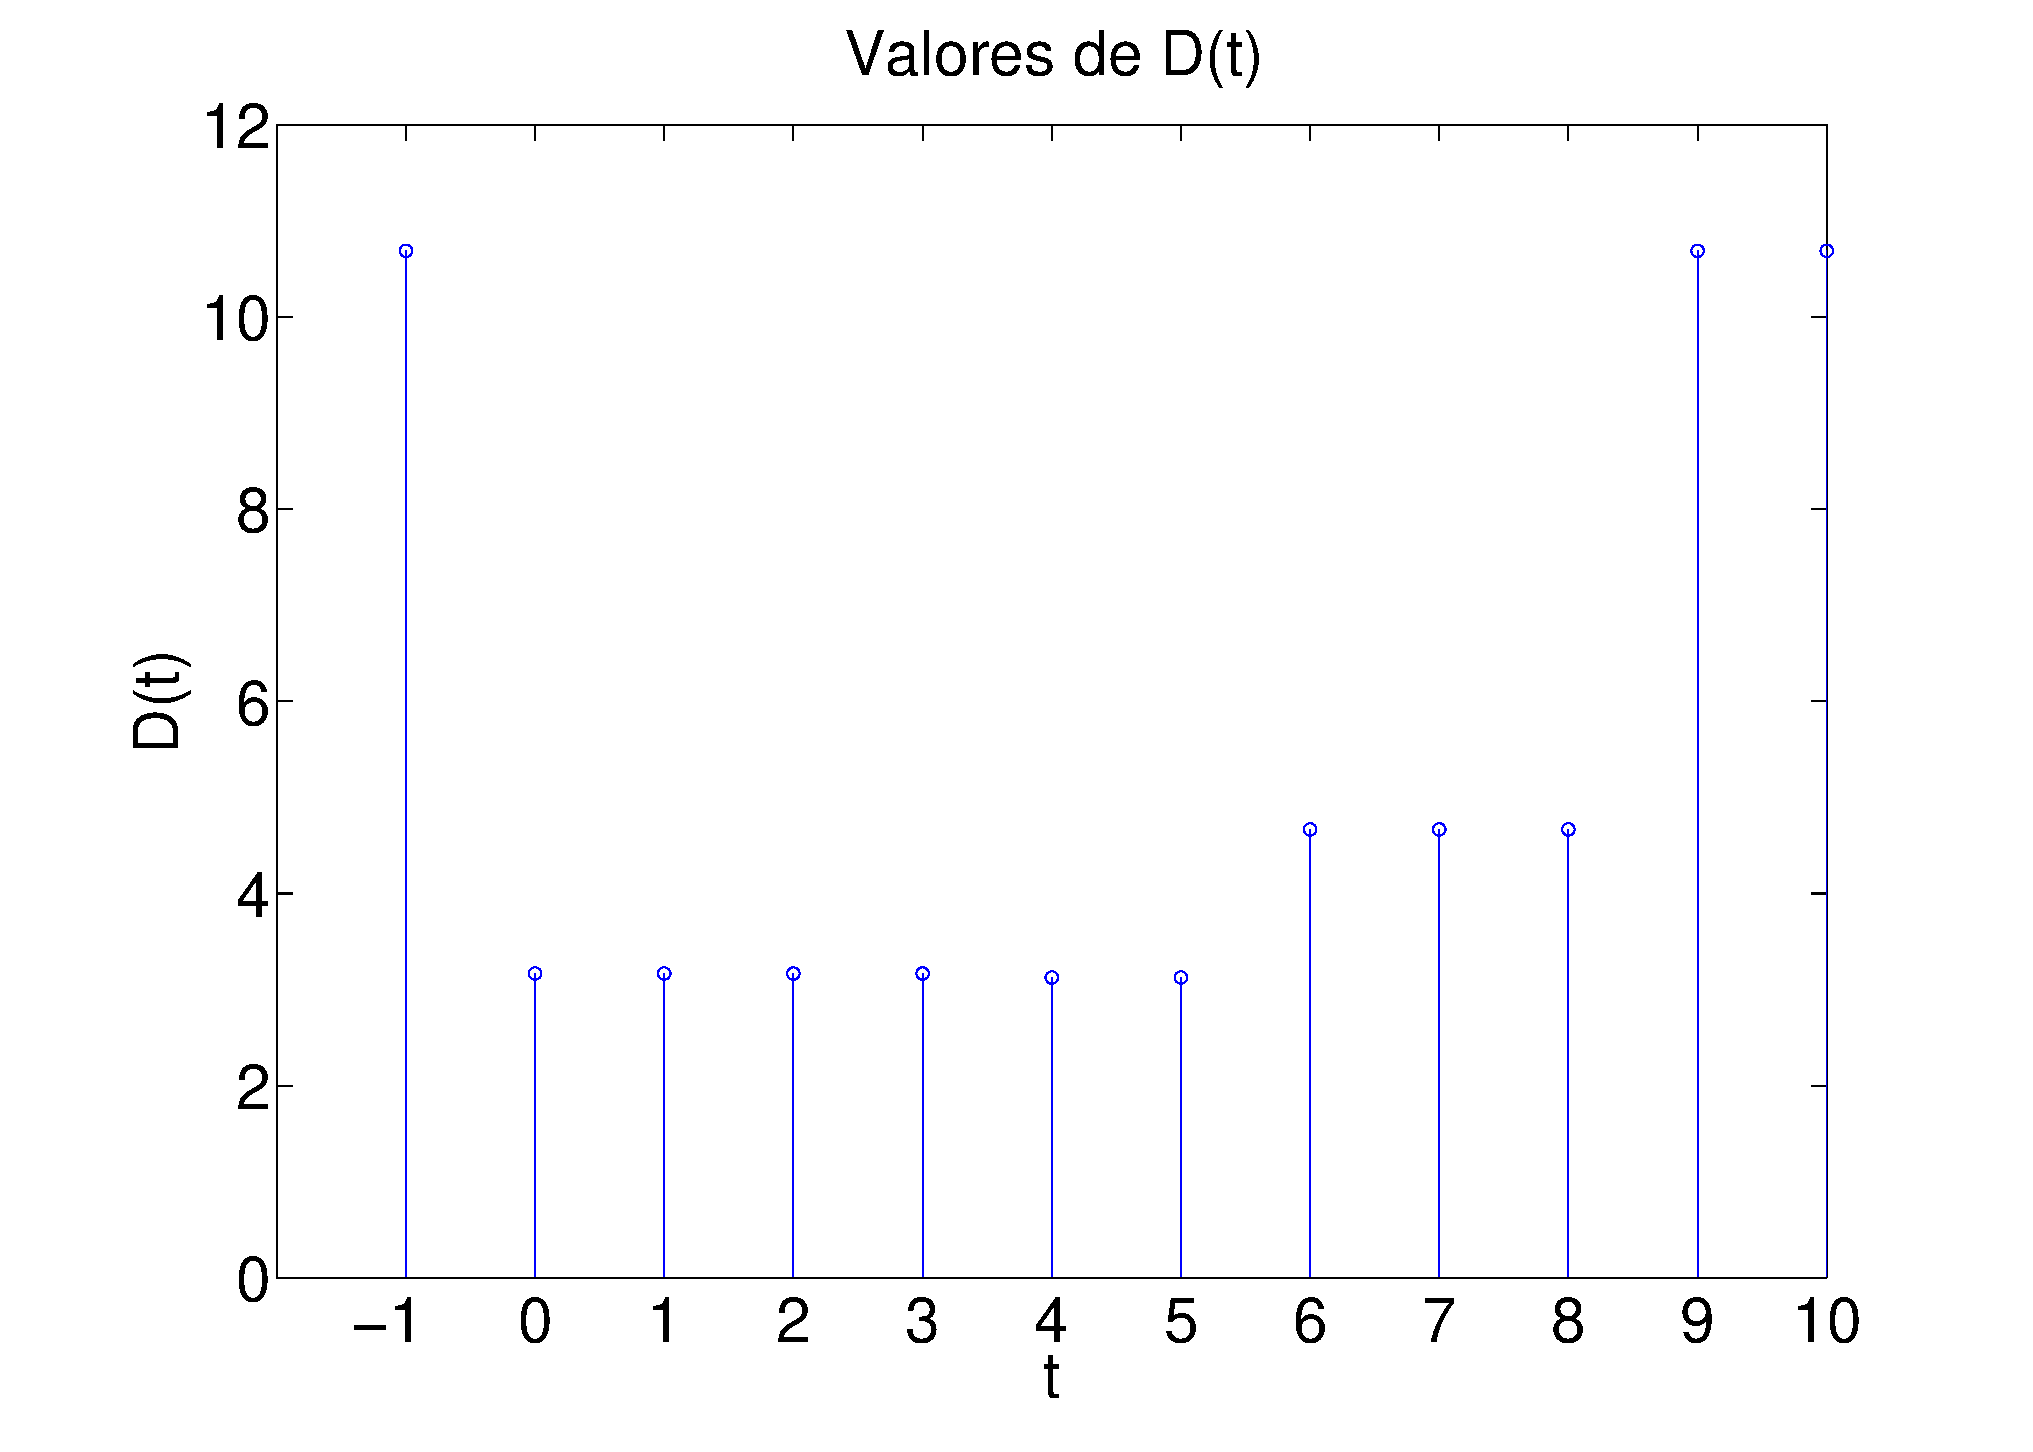
\includegraphics[width = 0.5\textwidth]{Q1_A_distorcao}
	\caption{Valores de $D(t)$}
	\label{grafico_distorcao}
\end{figure}

\textbf{b) Considere centros de massa com valores iniciais dados por $y_1 = 3,0$ e $y_2 = 3,4$. Calcule a matriz de probabilidade $p(y|x)$, assumindo $T = 1,0$.}\\

\paragraph{} Nesse item, a condição de ``Hard Clustering" {} não é mais assumida. Agora, o problema de associação é tratado como um \emph{``Soft Clustering"}, i. e., cada amostra é associada a cada grupo possível segundo uma probabilidade, em uma dada temperatura $T$. A função custo a ser minimizada, considerando o ``Soft Clustering", não é mais, somente a função $D$, e sim a associação de duas funções: a função de distorção $D$ e a função de entropia $H$, segundo a Equação \eqref{eq_funcao_custo}.\\

\begin{equation}\label{eq_funcao_custo}
J = D - TH
\end{equation}

\paragraph{} Sendo assim, a minimização da função custo ocorre em duas etapas: primeiro, maximiza-se a entropia do problema (o termo $-TH$) e, depois, minimiza-se a distorção (o termo $D$). Reduzindo a temperatura $T$ e aplicando esse mesmo procedimento a cada uma, é garantido que o mínimo alcançado será o global.\\

\paragraph{} O primeiro passo, então, é efetuado. Para se maximizar a entropia, deve-se achar a matriz de probabilidade $p(y|x)$ que gera essa condição. Ela pode ser encontrada através da aplicação da Equação \eqref{eq_condicao_particao}, também conhecida como \emph{condição de partição}. As colunas dessa matriz correspondem às amostras $x$, ao passo que as linhas correspondem aos centróides $y$.\\

\begin{equation}\label{eq_condicao_particao}
p(y_j|x_i) = \frac{e^{-\frac{d(x_i,y_j)}{T}}}{\sum_y e^{-\frac{d(x_i,y)}{T}}}
\end{equation}

\paragraph{} A função $d(x,y)$ é a distância euclidiana entre a amostra $x$ e o centróide $y$. Portanto, para se efetuar o cálculo da condição de partição, é preciso inicializar os valores dos centróides, que, no caso, são $y_1 = 3,0$ e $y_2 = 3,4$. Por exemplo, a distância da amostra $x = 0$ para os centróides $y_1$ e $y_2$ é dada por:\\

\begin{equation}\label{eq_distancia_amostra0_centroides}
\begin{cases}
	d(0,3) = (0-3)^2 = 9\\
	d(0,3,4) = (0-3,4)^2 = 11,56
\end{cases}
\end{equation} 

\paragraph{} Substituindo a Equação \eqref{eq_distancia_amostra0_centroides} em \eqref{eq_condicao_particao}, chega-se ao seguinte valor:\\

\begin{equation}
p(y_1 = 3|x_1 = 0) = \frac{e^{-\frac{d(0,3)}{T}}}{e^{-\frac{d(0,3)}{T}} + e^{-\frac{d(0,3,4)}{T}}} = \frac{e^{-\frac{9}{1}}}{e^{-\frac{9}{1}} + e^{-\frac{11,56}{1}}} \approx 0,9282 
\end{equation}

\paragraph{} Vale ressaltar que a soma dos elementos de cada coluna da matriz devem sempre igualar 1, uma vez que elas tratam das probabilidades de se associar uma certa amostra a um determinado grupo. Aplicando esse mesmo cálculo para cada amostra e grupo, obtém-se, então, a matriz $p(y|x)$, exibida abaixo:\\

\begin{equation}
p(y|x) = \left[\begin{array}{cccc}
0,9282 & 0,3452 & 0,0962 & 0,0096 \\ 
0,0718 & 0,6548 & 0,9038 & 0,9904
\end{array} \right]
\end{equation}\\

\textbf{c) Utilizando $p(y|x)$ do item (b), calcule o valor de $D$ a partir da expressão $\sum_x p(x) \sum_y p(y|x)d(x,y)$.}\\

\paragraph{} Utilizando a expressão dada, substituindo $p(x) = 1/4$ (já que os dados $x$ são equiprováveis), $p(y|x)$ pela matriz calculada anteriormente e $d(x,y)$ pelas respectivas distâncias de cada amostra $x$ a cada centróide $y$, obtém-se $D \approx 12,0361$. É interessante notar que esse valor obtido não corresponde ao menor valor de $D$ encontrado no item (a). Isso, no entanto, não configura um erro no procedimento de minimização, já que, conforme dito anteriormente, no item (b), buscou-se maximizar o termo $-TH$ da função custo $J$, o que não significa que o termo $D$ também será minimizado. Até então, o termo $D$ sequer foi considerado no procedimento de minimização de $J$. Isso será feito no passo seguinte.\\

\textbf{d) Utilizando $p(y|x)$ do item (b), calcule valores atualizados para os centros de massa $y_1$ e $y_2$.}\\

\paragraph{} Com a matriz $p(y|x)$ calculada e a entropia $H$ maximizada, inicia-se o segundo passo na minimização de $J$, que consiste em minimizar o termo $D$, correspondente à distorção, ou ao erro médio quadrático. A ideia por trás desse passo é simples: uma vez definida a distribuição das associações, sabe-se quais amostras são mais prováveis de estarem associadas a um determinado grupo. Por meio dessa informação, é possível posicionar melhor os centróides, de forma a minimizar a distância das amostras para eles e, com isso, minimizar o valor da função $D$. A Equação \eqref{eq_cond_centroide}, responsável por encontrar esse valor mínimo, é denominada \emph{``condição de centróide"}:\\

\begin{equation}
\sum_x p(x,y) \frac{\partial}{\partial y}d(x,y) = 0
\end{equation}\\

\paragraph{} Expandindo $p(x,y) = p(y|x)p(x)$ e sabendo que, nesse caso, $p(x) = \frac{1}{N} = \frac{1}{4}$:\\

\begin{equation}
\frac{1}{4} \sum_x p(y|x) \frac{\partial}{\partial y} d(x,y) = 0, \quad \forall y \in Y
\end{equation}\\

\paragraph{} Como, nesse caso, $d(x,y)$ corresponde à distância euclidiana entre os pontos $x$ e $y$, os centróides $y_1$ e $y_2$ são determinados pela Equação \eqref{eq_centroides}:\\

\begin{equation}\label{eq_centroides}
	y_j = \frac{\sum_i p(y_j|x_i)x_i}{\sum_i p(y_j|x_i)}
\end{equation}\\

\paragraph{} Usando a Equação \eqref{eq_centroides}, substituindo pelos valores correspondentes, chega-se aos seguintes valores para os centróides: $y_1 = 1,4822$ e $y_2 = 6,4698$.\\

\textbf{e) Repita os itens (b), (c), e (d) utilizando $T = 0,1$.}\\

\paragraph{} Os valores das variáveis de cada item, para $T = 0,1$, estão exibidas abaixo.\\

\begin{equation*}
p(y|x) = \left[\begin{array}{cccc}
1 & 0,0017 & 0 & 0 \\ 
0 & 0,9983 & 1 & 1
\end{array} \right]
\end{equation*}\\

\begin{equation*}
D = 11,8703
\end{equation*}\\

\begin{equation*}
\begin{cases}
	y_1 = 0,0066\\
	y_2 = 6,3346\\
\end{cases}
\end{equation*}

\textbf{f) Repita os itens (b), (c), e (d) utilizando $T = 50$.}\\

\paragraph{} Os valores das variáveis de cada item, para $T = 50$, estão exibidas abaixo.\\

\begin{equation*}
p(y|x) = \left[\begin{array}{cccc}
0,5128 & 0,4968 & 0,4888 & 0,4768 \\ 
0,4872 & 0,5032 & 0,5112 & 0,5232
\end{array} \right]
\end{equation*}\\

\begin{equation*}
D = 13,0881
\end{equation*}\\

\begin{equation*}
\begin{cases}
	y_1 = 4,6635\\
	y_2 = 4,8344\\
\end{cases}
\end{equation*}\\

\textbf{g) Compare os resultados obtidos nos itens (d), (e), e (f).}\\

\paragraph{} Quando se utiliza baixas temperaturas, como no caso de $T = 0,1$, o segundo termo da função de custo $J$, referente à entropia ($-TH$), torna-se muito menor do que o primeiro, referente à distorção ($D$). O problema, então, passa a se tornar bem mais próximo de um ``Hard Clustering", como se verifica através da matriz de probabilidade $p(y|x)$. Com isso, a minimização de $J$ é quase totalmente correspondente à minimização da função $D$. A Figura \ref{disposicao_centroides_t_pequeno} mostra como ficam organizados os centróides nesse caso. Note que a amostra mais distante das demais ($x = 0$) passa a compor um único grupo, tendo o centróide localizado muito próxima da amostra. Isso é uma consequência direta da matriz de probabilidade $p(y|x)$, nessa temperatura. As outras amostras compõem o outro grupo.\\

\begin{figure}[H]
	\centering
	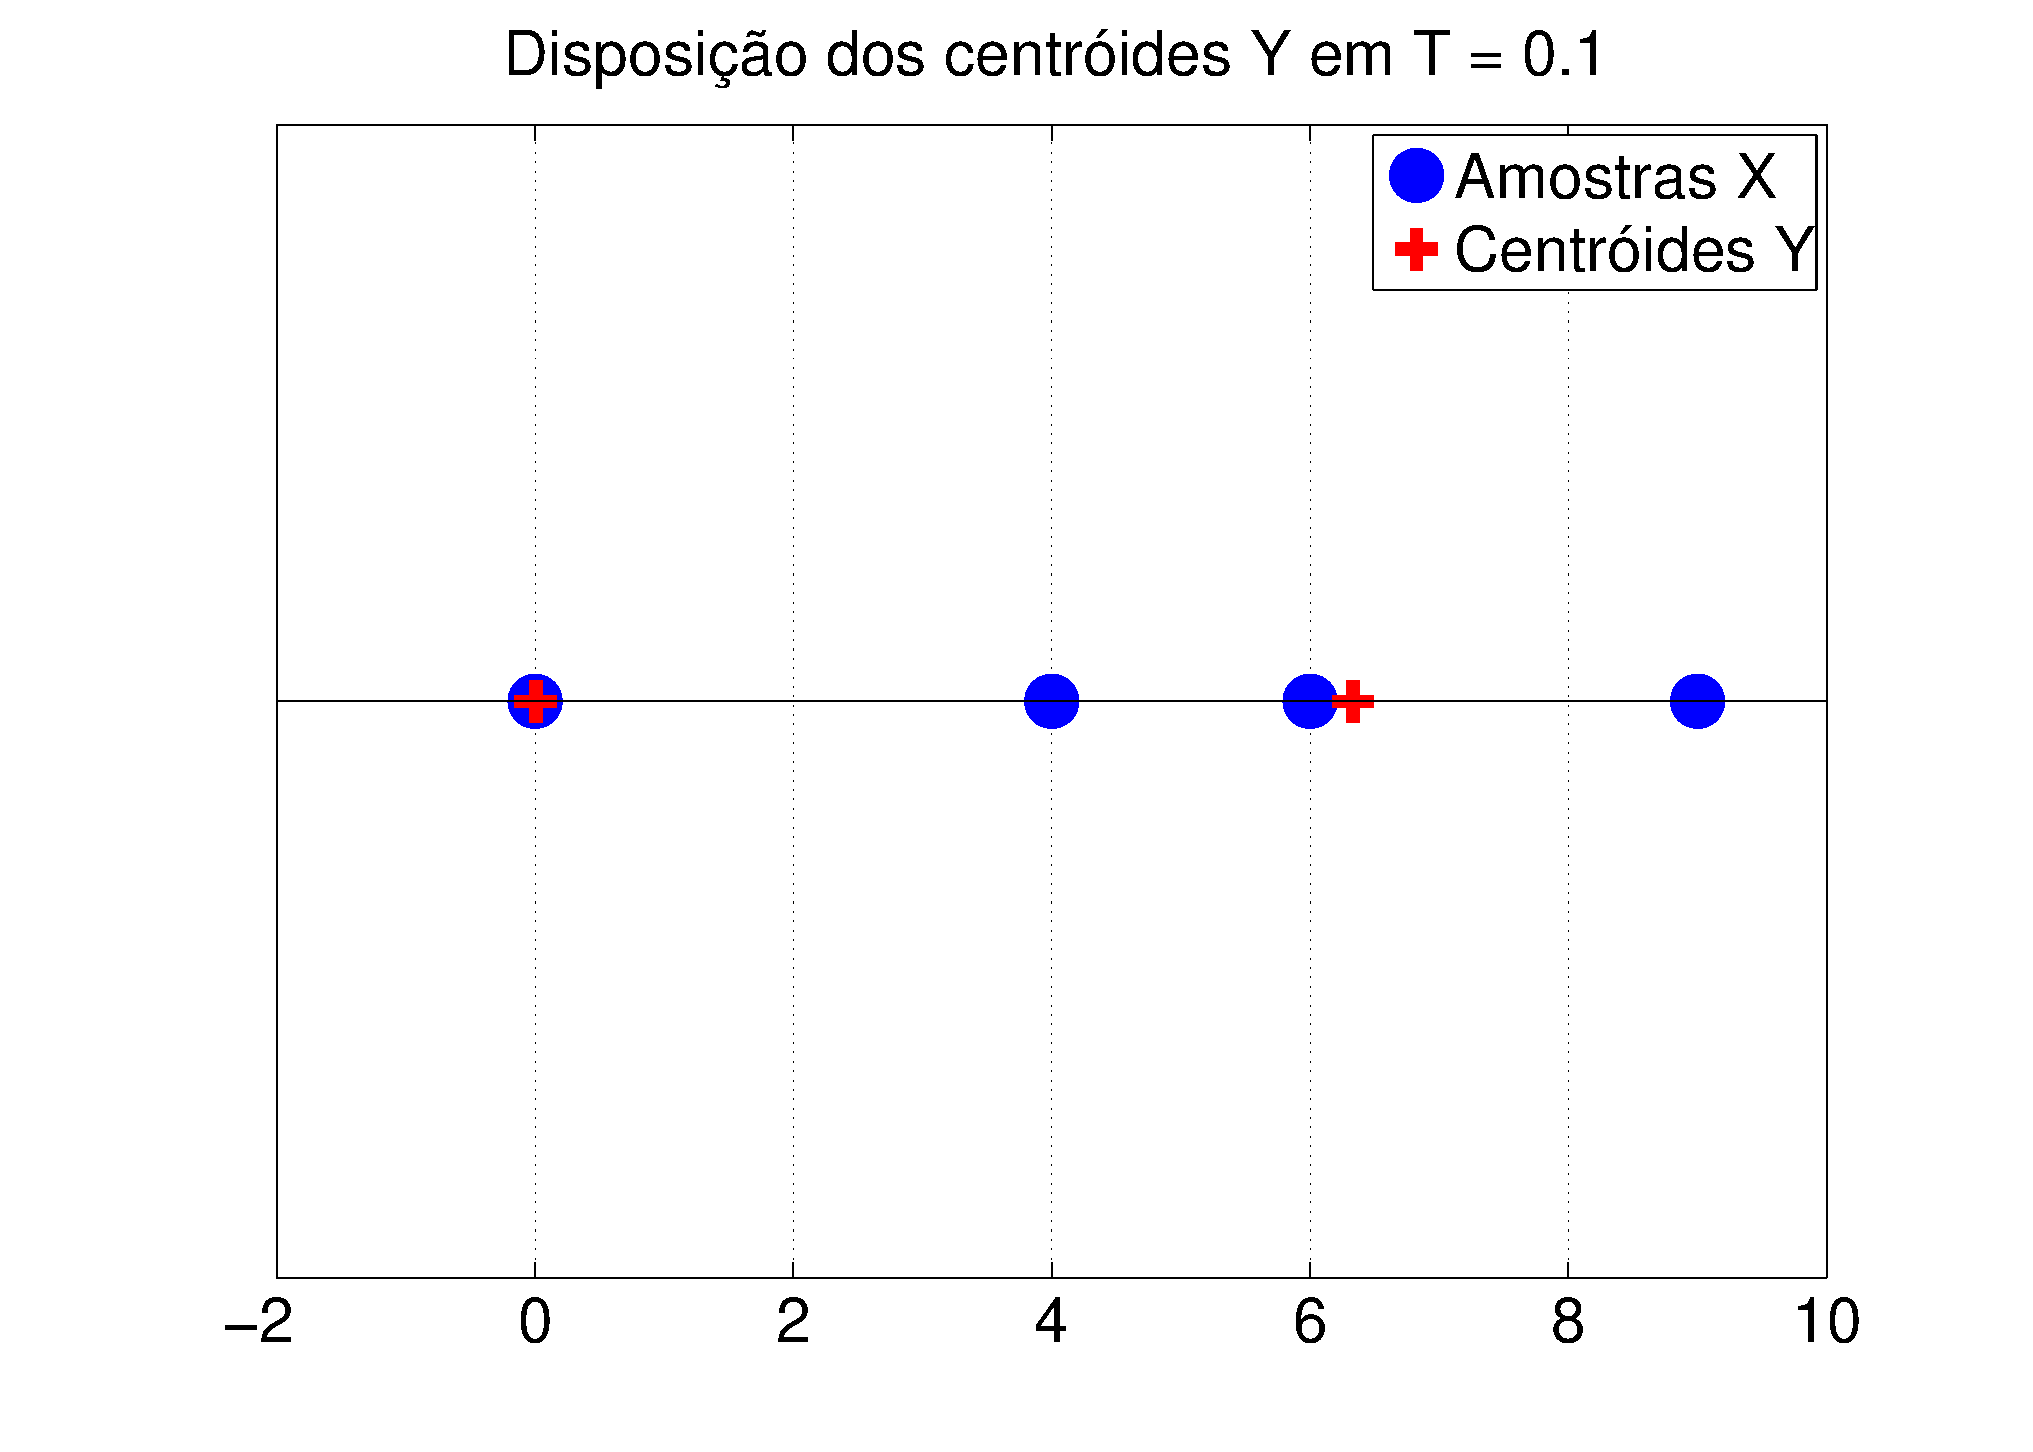
\includegraphics[width = 0.5\textwidth]{Q1_G_centroides_t_pequeno}
	\caption{Disposição dos centróides para $T = 0,1$}
	\label{disposicao_centroides_t_pequeno}
\end{figure}

\paragraph{} Por outro lado, quando a temperatura é alta, o termo $-TH$ passa a dominar a expressão da função custo, de modo que ele tem um impacto muito superior na minimização da função, do que o primeiro termo $D$. Consequentemente, é possível observar na Figura \ref{disposicao_centroides_t_grande} que ambos os centróides localizam-se muito próximos um do outro. A associação de uma amostra a um grupo é tão incerta que, analisando a matriz $p(y|x)$ para essa temperatura, nota-se que as probabilidades de associação de cada amostra a cada grupo é próxima de 50\%. Essa grande aleatoriedade ilustra o conceito de entropia. No caso extremo, em que $T \rightarrow \infty$, os dois centróides são coincidentes e a aleatoriedade é máxima, i.e., cada amostra tem chances iguais de serem associadas a cada grupo (no caso, 50\%).\\

\begin{figure}[H]
	\centering
	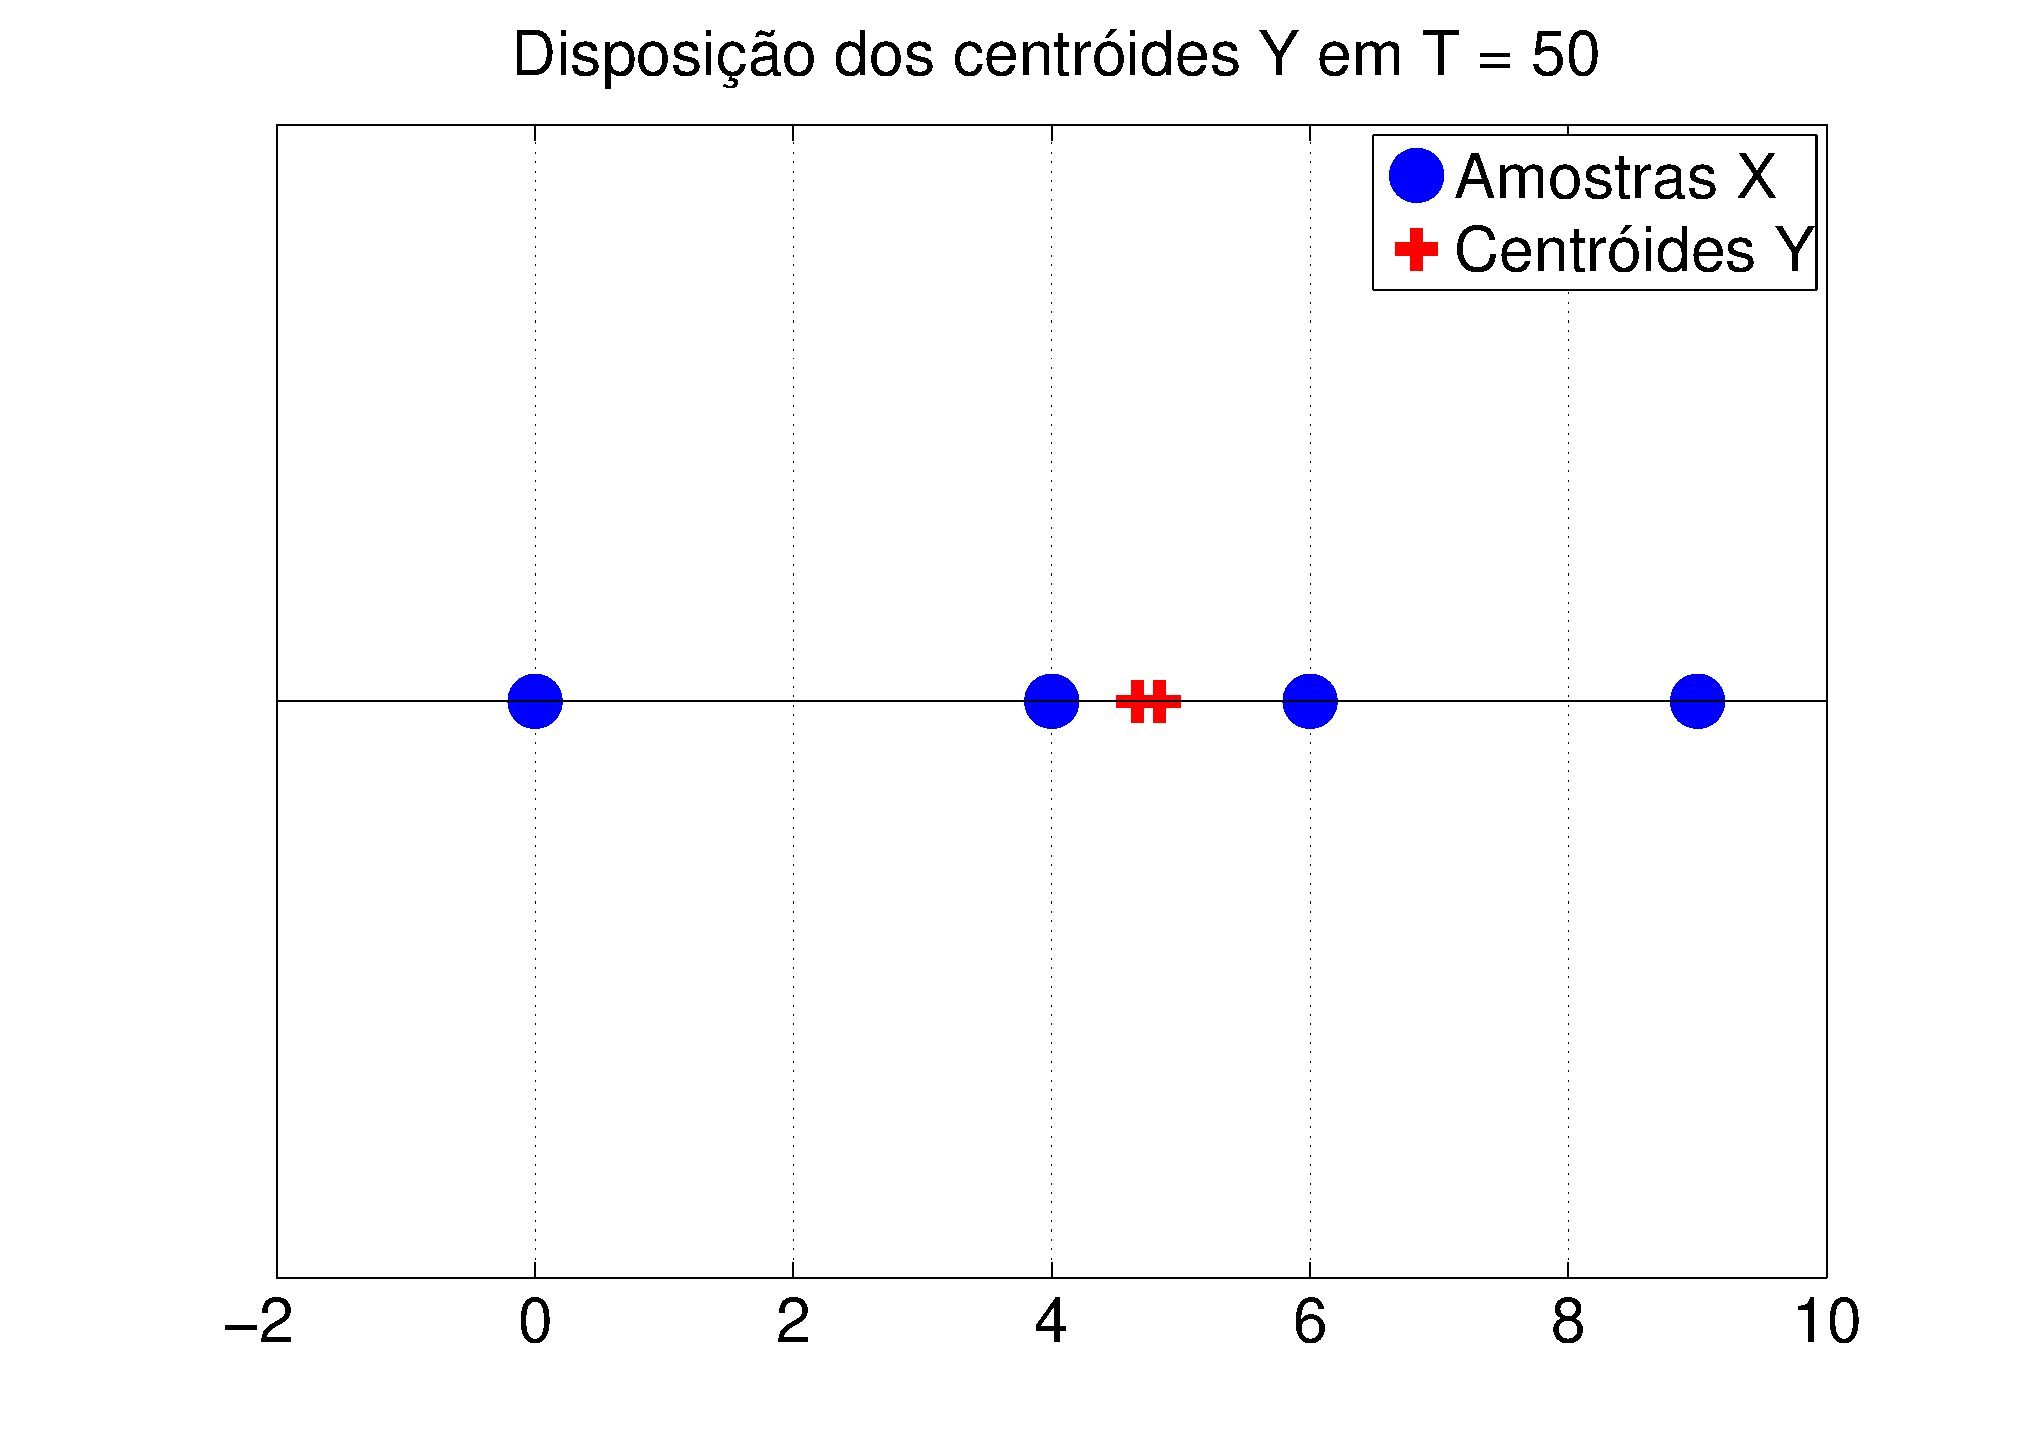
\includegraphics[width = 0.5\textwidth]{Q1_G_centroides_t_grande}
	\caption{Disposição dos centróides para $T = 50$}
	\label{disposicao_centroides_t_grande}
\end{figure}

\section*{Questão 2}

\textbf{Proponha uma função $J(\text{\textbf{x}})$, sendo \textbf{x} um vetor com 20 dimensões, cujo ponto mínimo você conheça. Evite propor funções que tenham um só ponto mínimo. Encontre o ponto mínimo global utilizando S.A.}\\

\textbf{Obs.: neste exercício, entregue o código utilizado e alguns comentários sobre o resultado obtido.}\\

\paragraph{} A função custo escolhida para se otimizar um polinômio de alto grau, o qual contém 3 mínimos (2 locais e 1 global). O mínimo global vale 0 e localiza-se na origem do espaço de dimensão $\mathbb{R}^{20}$. A Figura \ref{funcao_custo} mostra a forma dessa função no espaço 2-D.\\

\begin{figure}[H]
	\centering
	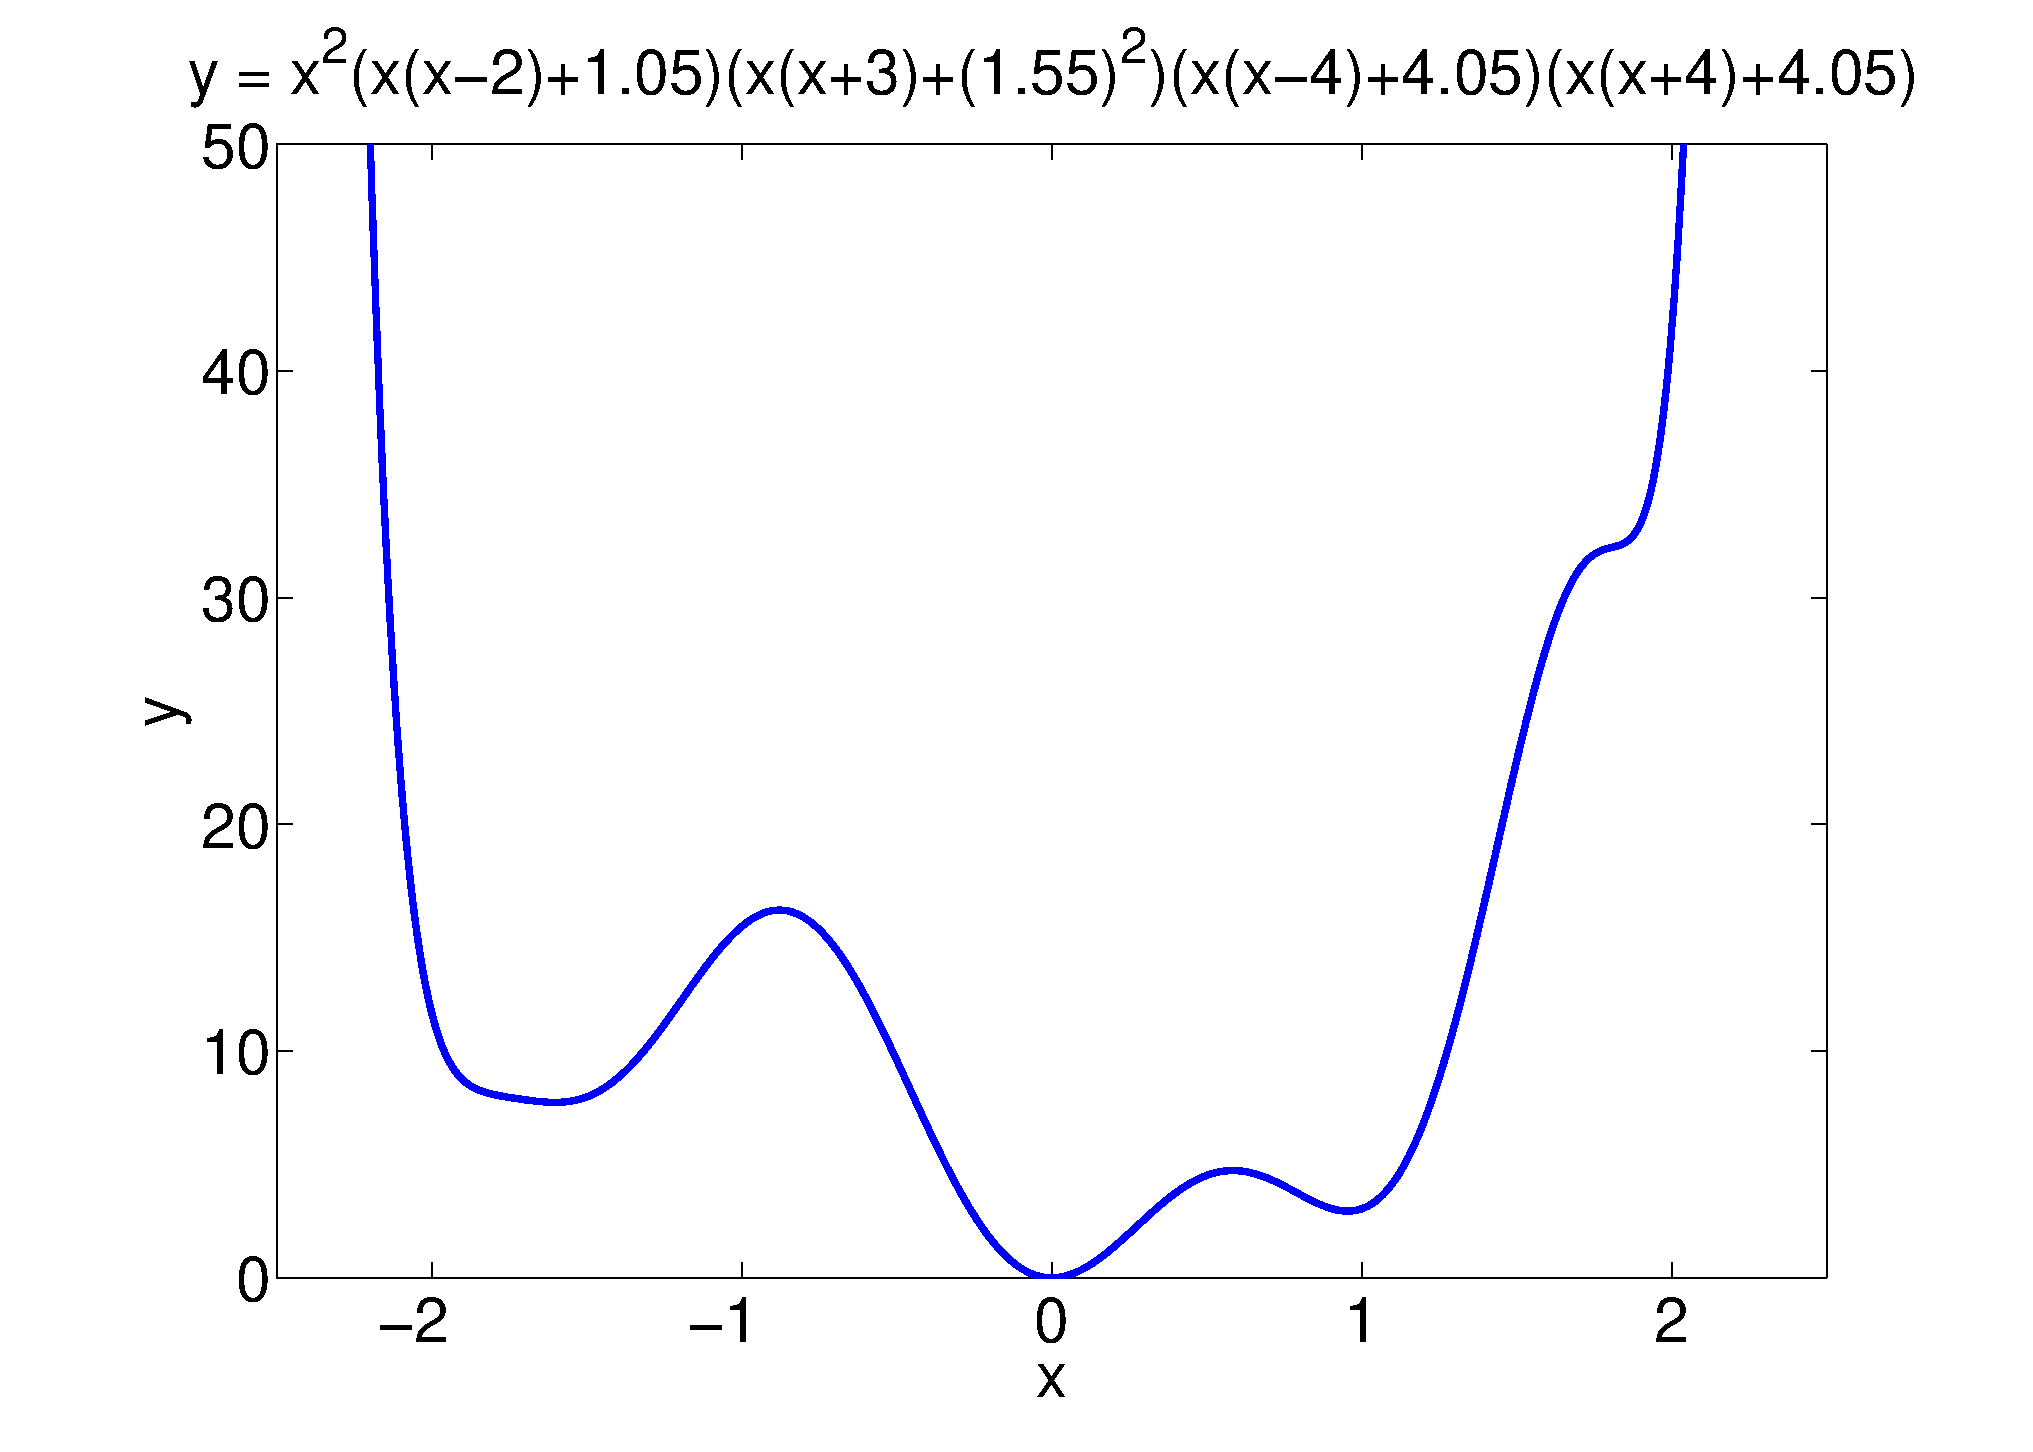
\includegraphics[width=0.5\textwidth]{Q2_funcao_J_2D}
	\caption{Exemplo da função custo $J(x)$ de uma variável}
	\label{funcao_custo}
\end{figure}

\paragraph{} Para facilitar a leitura da função $J(\text{\textbf{x}})$, estão expostos abaixo os polinômios que foram combinados para gerar a função custo final.\\

\begin{equation*}
\begin{cases}
	f_1(\text{\textbf{x}}) = \sum_i x_i^2\\
	f_2(\text{\textbf{x}}) = \sum_i \left(x_i \times (x_i - 2)+1,05\right)\\
	f_3(\text{\textbf{x}}) = \sum_i \left(x_i \times (x_i - 3)+(1,55)^2\right)\\
	f_4(\text{\textbf{x}}) = \sum_i \left(x_i \times (x_i - 4)+4,05\right)\\
	f_5(\text{\textbf{x}}) = \sum_i \left(x_i \times (x_i + 4)+4,05\right)
\end{cases}, \quad i = 1,2,...,20
\end{equation*}\\

\begin{equation*}
J(\text{\textbf{x}}) = f_1(\text{\textbf{x}}) \times f_2(\text{\textbf{x}}) \times f_3(\text{\textbf{x}}) \times f_4(\text{\textbf{x}}) \times f_5(\text{\textbf{x}})
\end{equation*}\\

\paragraph{} O código, em MATLAB, que implementa a solução para o item em questão encontra-se a seguir:\\

\begin{lstlisting}
T = zeros(1,10);
T0 = 1;
for i = 1:10
    T(i) = T0/i;
end

N = 1000000;
epsilon = 0.05;
x_atual = random('unif', -2,2,20,1);

f1 = sum((x_atual.^2));
f2 = sum((x_atual.*(x_atual-2)+1.05));
f3 = sum((x_atual.*(x_atual+3)+(1.55)^2));
f4 = sum((x_atual.*(x_atual-4)+4.05));
f5 = sum((x_atual.*(x_atual+4)+4.05));

J_atual = f1 .* f2 .* f3 .* f4 .* f5;
J_min = J_atual;

J = zeros(length(T), N);
X = zeros(size(x_atual,1),N,length(T));

for k = 1:length(T)
    for n = 1:N
        
        r = trnd(1,size(x_atual));
        
        x_futuro = x_atual + epsilon * r;
        
        f1 = sum((x_futuro.^2));
        f2 = sum((x_futuro.*(x_futuro-2)+1.05));
        f3 = sum((x_futuro.*(x_futuro+3)+(1.55)^2));
        f4 = sum((x_futuro.*(x_futuro-4)+4.05));
        f5 = sum((x_futuro.*(x_futuro+4)+4.05));
        
        J_futuro = f1 .* f2 .* f3 .* f4 .* f5;
        
        delta_J = J_futuro - J_atual;
        
        if delta_J < 0
            x_atual = x_futuro;
            J_atual = J_futuro;
        else
            a = rand();
            
            if a < exp(-(delta_J)/T(k))
                x_atual = x_futuro;
                J_atual = J_futuro;
            end
        end
        
        if J_atual < J_min
            J_min = J_atual;
            X_min = x_atual;
        end
        
        J(k,n) = J_atual;
        X(:,n,k) = x_atual;
        
    end
end
            
\end{lstlisting}

\paragraph{} Conforme a dimensão do problema cresce, a convergência para o mínimo global torna-se mais demorada, já que os graus de liberdade aumentam (para esse item, por exemplo, tem-se 20 graus de liberdade). Isso pode ser observado nesse item. Quando \textbf{x} é um vetor de 1 dimensão (ou seja, um escalar), utilizando-se FSA (\emph{Fast Simulated Annealing}) com 10 temperaturas distintas e 1000 iterações em cada uma, alcança-se um valor muito próximo do mínimo global ($3.22 \times 10^{-9}$) (exibido na Figura \ref{fsa_2d}).\\ 

\begin{figure}[H]
	\centering
	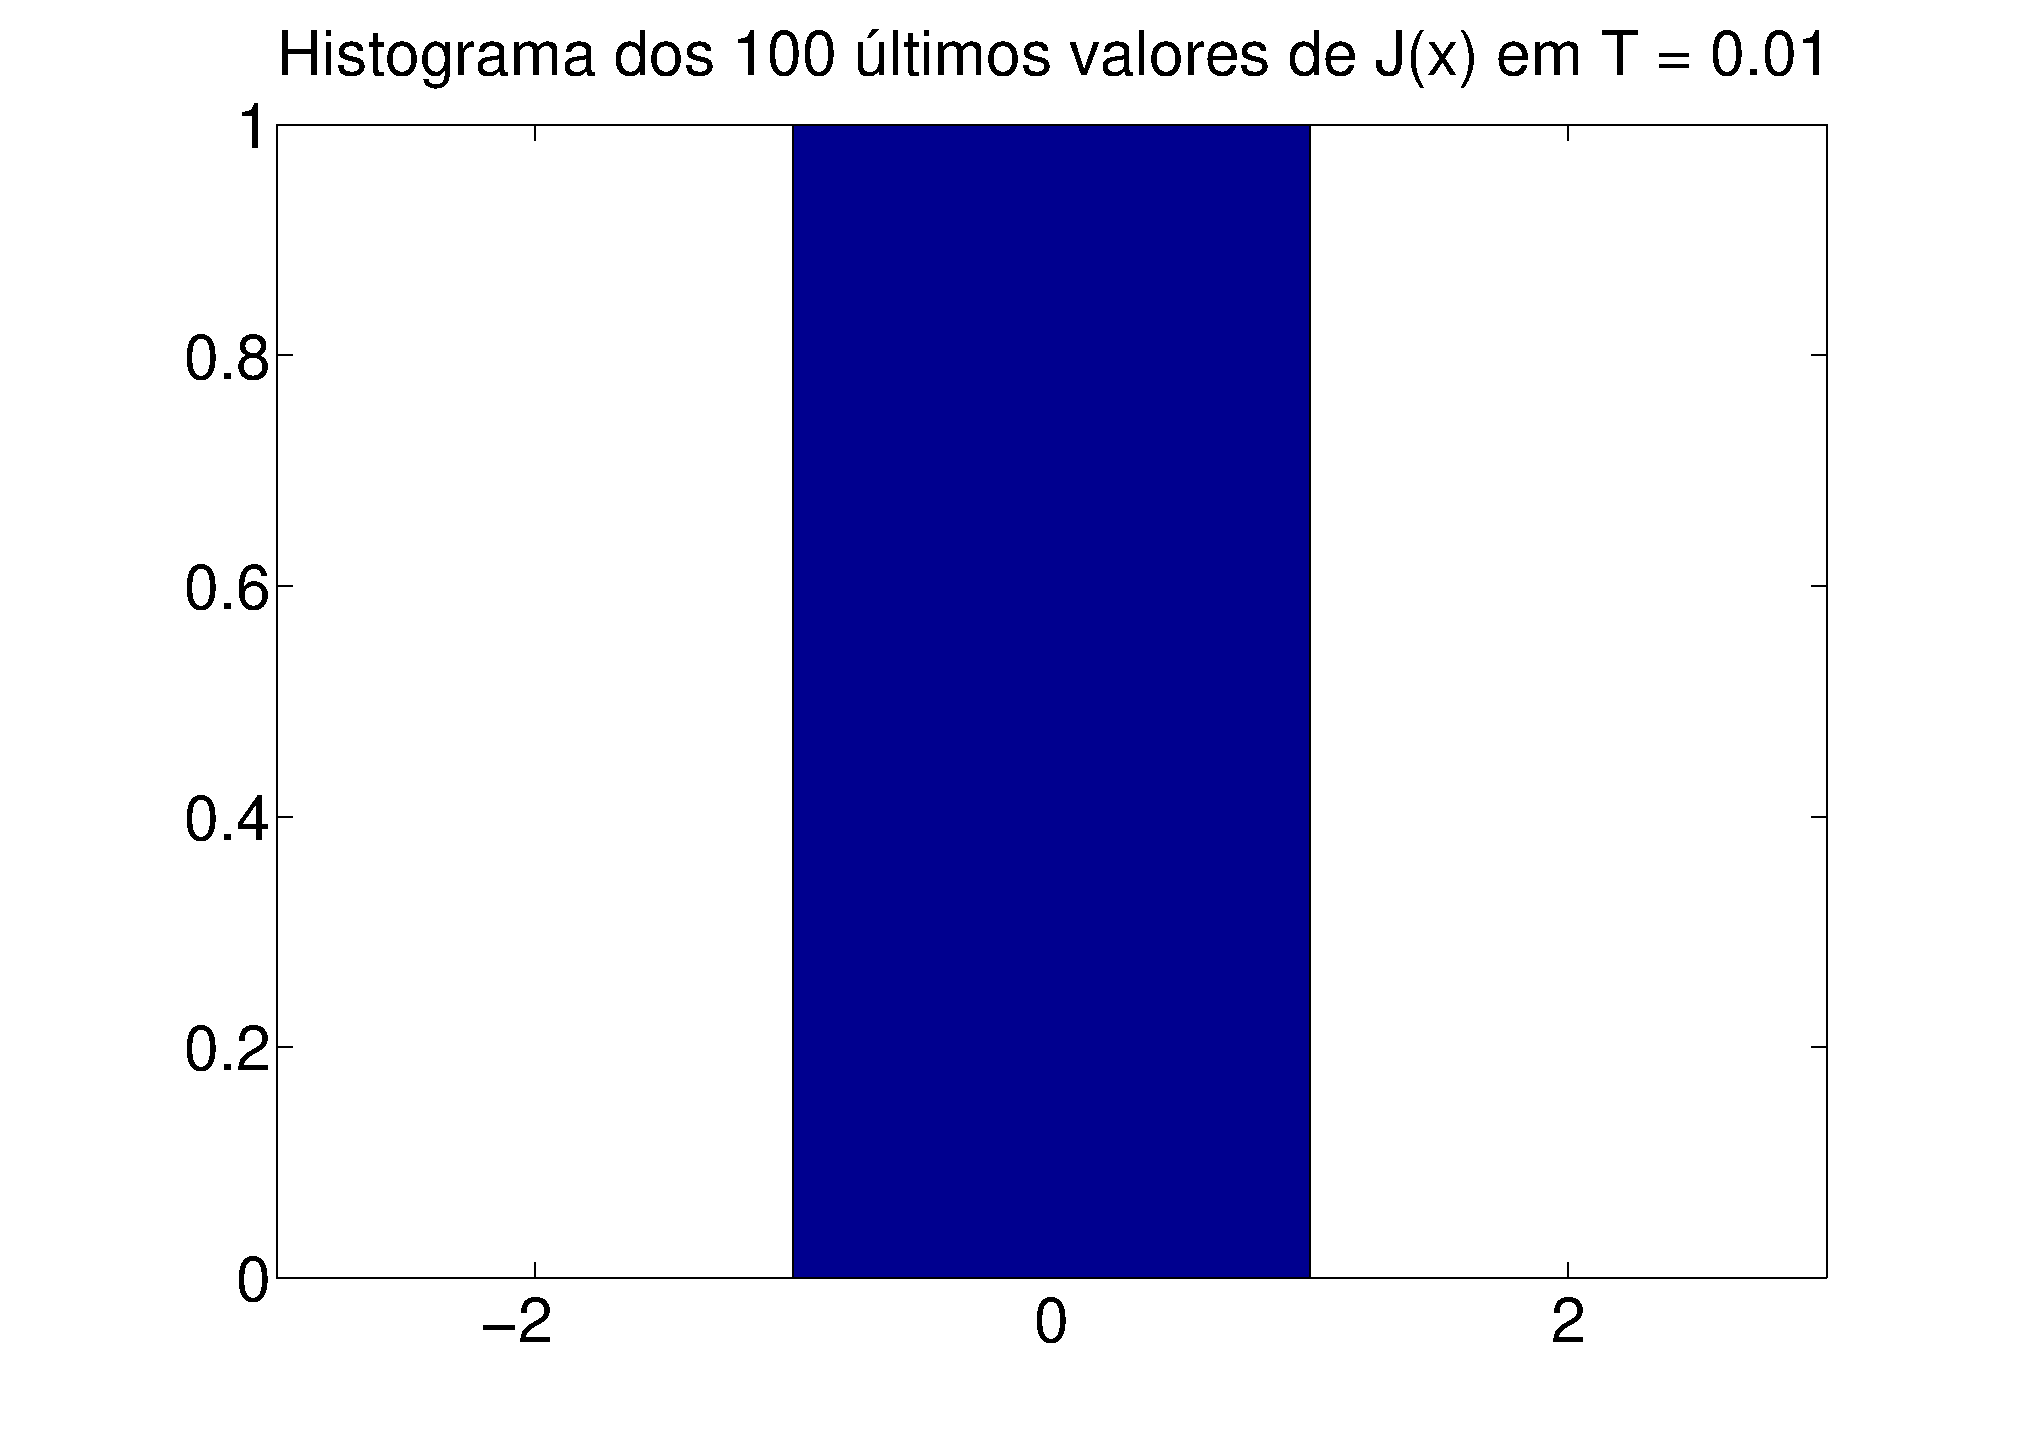
\includegraphics[width = 0.5\textwidth]{Q2_hist_J_uma_variavel}
	\caption{Histograma dos 100 últimos valores da função custo $J(x)$ de 1 variável em $T = 0,1$, aplicando FSA}
	\label{fsa_2d}
\end{figure}

\paragraph{} Agora, fazendo o vetor \textbf{x} de 20 dimensões e aplicando o FSA com 10 temperaturas distintas e 1000000 iterações em cada uma, o mínimo encontrado foi de 86964, o qual ainda encontra-se distante do mínimo global, que é 0. Isso ilustra como dimensões de alta ordem acarretam em um aumento considerável no tempo de convergência. Conforme são acrescentadas mais iterações e temperaturas, mais o algoritmo se aproxima do mínimo global. A Figura \ref{fsa_20_variaveis} mostra o histograma dos 100000 últimos valores da função custo $J(\text{\textbf{x}})$ na temperatura $T = 0,1$.\\

\begin{figure}[H]
	\centering
	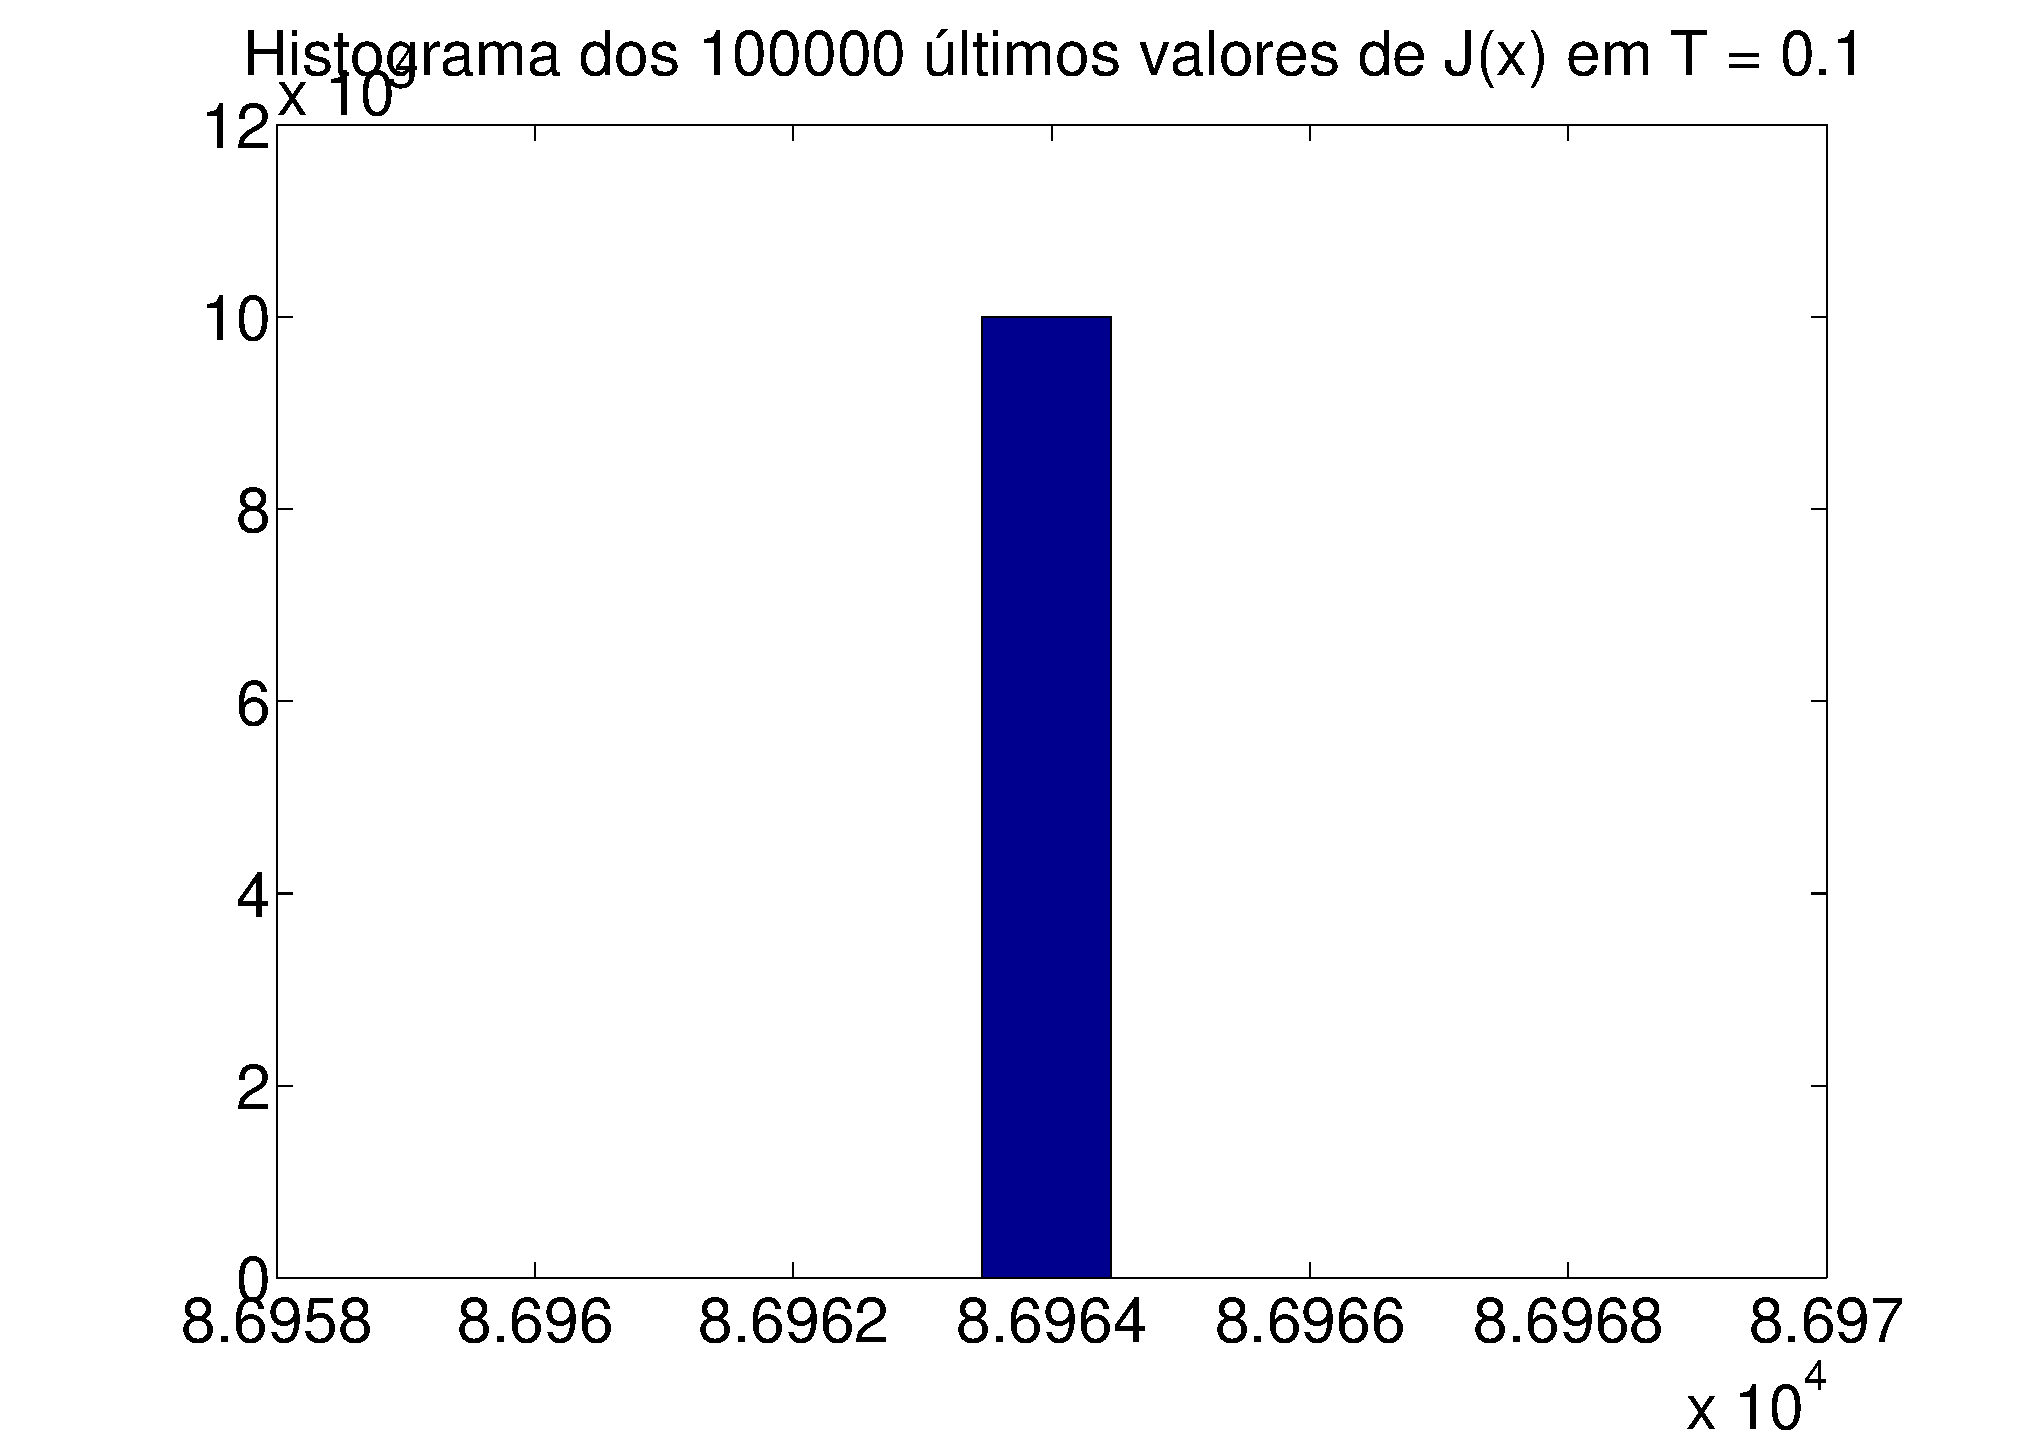
\includegraphics[width = 0.5\textwidth]{Q2_hist_J_vinte_variaveis_fsa}
	\caption{Histograma dos 100000 últimos valores de $J(\text{\textbf{x}})$ em $T = 0,1$}
	\label{fsa_20_variaveis}
\end{figure}

\end{document}